% !Mode:: "TeX:UTF-8"
%%==========================
%% chapter01.tex for SJTU Master Thesis
%% based on CASthesis
%% modified by wei.jianwen@gmail.com
%% version: 0.3a
%% Encoding: UTF-8
%% last update: Dec 5th, 2010
%%==================================================

%\bibliographystyle{sjtu2} %[此处用于每章都生产参考文献]
\chapter{人体姿势预测的应用案例}
\label{chap:app}
人体姿势检测是计算机视觉领域非常基础的一项工作,我们可以利用人体姿势预测的结果来解决很多其它实际问题,比如基于图片数据集相关的问题,
特别是那些专注在人物相关的问题。
在本章中,首先我们会介绍一下我之前的一篇事件挖掘的工作,我们的工作是基于图片数据集,从Flickr上抓取的人物日常生活照片。
由于以图片数据集作为背景,而且Flickr上的图片数据大部分是包含人物的,而事件挖掘就是要分析图片要表达的语义信息,
所以自然可以想到,我们可以利用人体姿势预测的结果来分析出图片中人物所表达的语义信息,从而进行事件挖掘。
其次,我们会介绍一下人体姿势预测在电商平台上(淘宝、亚马逊、eBay等)衣服搜索的应用。
服饰类商品在电商平台上占据了大量的份额,因此如何帮助人们尽快的找到自己喜欢的衣服是一个很大的挑战,
衣服搜索这项人物应运而生,它的核心就在于分析出图片中衣服的属性信息,然后通过属性信息去海量的衣服数据库中找出最匹配用户需求的衣服。
显而易见,人体姿势预测的结果很明显可以帮助我们去分析出图片中衣服的属性信息,从而进行衣服属性匹配,得到衣服搜索的结果。
最后,我们会介绍一下基于图片的广告推荐。
广告推荐是互联网界最热门的话题之一,它是很多互联网公司最赚钱的部门,广告推荐质量的好坏直接影响到公司整个财年的好坏。
很多传统的广告是基于文本信息,但是随着图片时代的到来,基于图片的广告推荐成为了我们当下最大的挑战。
特别是对于包含人物的图片,我们可以根据周围的语义信息,来推荐合适的产品,从而提高广告推荐的质量,进而为公司带来可观的收入。
下面我们以此来介绍人体姿势预测在这三个任务中的应用。

\section{基于多媒体数据的事件挖掘}
事件挖掘一直是很热门的一个课题,早在70年代就被提出,用来挖掘预测社会上的突发事件,比如地震、恐怖事件等。
随着互联网时代的到来,信息的产生和传播变得越来越迅速,互联网上发生了很多很多事情,如何快速的去挖掘甚至预测事件,是一个很大的挑战。
我们之前的一份工作就是考虑在社交图片分享网站Flickr上的事件挖掘问题。
Flickr目前是全球最大的图片社交分享网站,每天有大量的用户在上面分享图片,记录自己的个人生活,而这些图片里实际上包含了大量的事件信息。
比如奥运会、比赛、个人旅游等照片,如果我们能挖掘出其中的事件信息,那么对于用户图片的组织,甚至搜索引擎中结果的结构化展示都有极其强大的帮助。

\begin{figure}
\centering
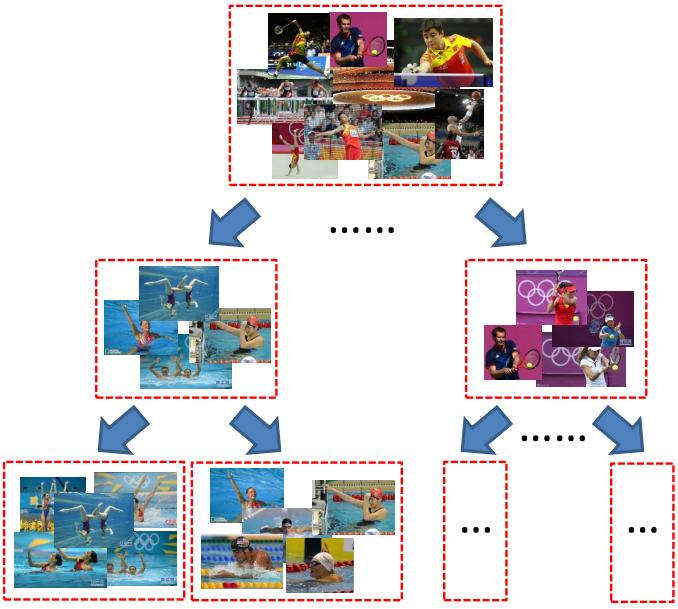
\includegraphics[width=0.9\textwidth]{img/lhed-example.pdf}
\caption{层次化事件例子}
\label{fig:lhed}
\end{figure}

对于事件来说,我们定义它为:在特定时间,特定地点,发生的某件事情。而这件事件的内容往往跟人物有很大关系,比如奥运会、登高比赛等。
本质上来说,事件挖掘是一种聚类的工作,需要分析任意两个图片之间在语义上的相似度,首先是不是跟事件相关,其次是不是代表同一个事件。
所以如何去判断图片之间的相似度是我们工作中最具挑战性的工作。
传统的做法可以通过图片周边信息(标签、标题、描述等)来描述相似度,或者通过图片的内容特征信息(颜色、纹理特征等)去描述相似度。
那么其实我们可以通过人体姿势预测的结果来帮助分析图片中人物的工作语义信息,比如运动、比赛、睡觉等。

我们的方法可以简单描述如下:针对每一张图片,我们检测出图片中人物的姿势(包括每个人体部位的位置和方向等),通过姿势信息,
我们可以判断出人物的动作语义信息,比如在运动或参加什么活动等,以及分析出人物所穿衣服的属性,通过衣服属性也可以得到更进一步的语义信息。
然后,我们将这些语义信息作为特征加入到对应的两张图片的相似度匹配中,就可以计算出比传统方法更精确的相似度。
进而我们可以利用聚类算法,将相似的图片聚集在一起,从中挖掘出事件。



通过上述方法,我们可以将人体姿势预测的结果利用到基于图片的事件挖掘中,通过人体姿势预测的结果挖掘出更深刻的两张图片之间的语义信息,
进而更精确的去描述两张图片之间的相似度,有利于精确的图片聚类,从而发现出对应的事件。

更进一步,我们可以发现事件之间也有层次化关系,比如奥运会这个事件,和奥运会上刘翔夺冠这个事件就是有层次关系的,前一个事件是后一个事件的父事件。
层次化事件的挖掘也是一个很有意思的课题,需要一个层次化聚类的算法去解决这个问题。
但其实核心的问题还是如何去层次化的描述两张图片之间的相似度。
对于更细时间尺度的事件挖掘来说,需要更精确的相似度匹配算法,也就是说我们需要对图片的内容了解的更多,
而人体姿势预测的结果为我们带来了更精细的信息。
因此,我们可以通过这种方式来更精确地挖掘真实世界中的层次化事件。

\begin{figure}
\centering
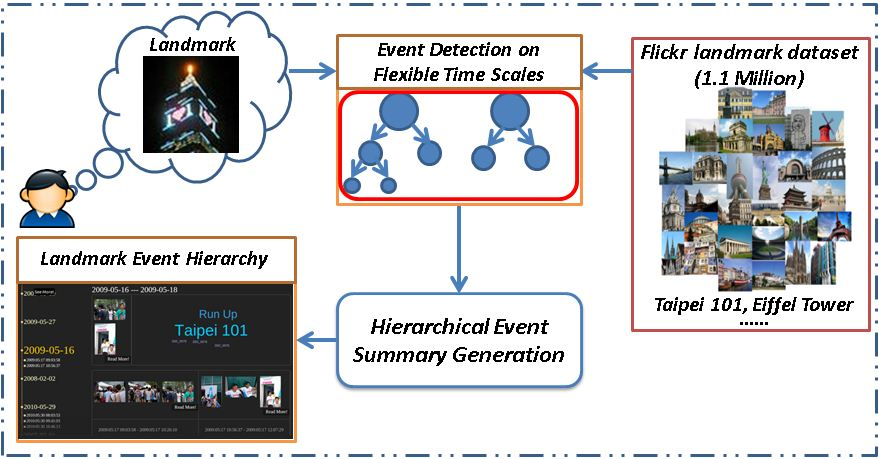
\includegraphics[width=0.9\textwidth]{img/architecture.jpg}
\caption{层次化事件挖掘流程图}
\label{fig:architecture}
\end{figure}

当然,对于视频数据集的事件挖掘也是比较容易的,因为视频本质上就是每秒24张图片,它是一个时间序列的图片数据,本质上来说,
就是时间序列约束下的图片数据集,可以采用我们的方法继续去解决。
更进一步,还可以利用HMM(隐式马尔可夫模型)去构建模型来对相邻时间点的图片关系进行预测。


\section{基于电商平台的衣服搜索}
电子商务越来越成为互联网界最重要的产业,随着阿里巴巴的上市,国内电子商务的力量逐渐被大大的呈现出来。
随之而来的是,中国更多的人拥有了就业机会,中国更多的人通过互联网购买到了最先进最实惠的产品,中国人民的需求被大大的挖掘出来。
服装类商品一直是商业社会中非常重要的产品,在电子商务中,人们一半以上的购物需求基本都是围绕着服装类商品展开。
而现在随着互联网信息的极度膨胀,如果在浩如烟海的电子商务平台上找到自己称心如意的服装,成为一个极大的挑战。
很多时候,我们都觉得上淘宝这样的网站,太过于复杂了。
一想起要搜索一个关键词,然后罗列了100多页的商品供用户选择,用户就会觉得极度的烦恼。本质上一个关键词很难反应用户真实的需求,
因此就会有很多次搜索请求,还很难真正得到用户想要的衣服商品。
如果有基于图片的衣服搜索引擎,那么将会大大减少用户的购买时间。
因为图片比关键词可以表达更丰富的信息,图片中包含了各种各样的显示信息,更容易满足用户的真正需求。
所以,如何去设计一个基于多媒体数据的衣服搜索引擎,就成为如今电子商务平台的一大挑战。

\begin{figure}
\centering
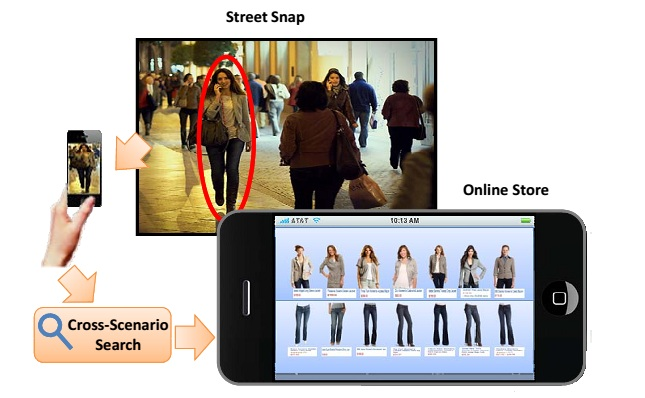
\includegraphics[width=0.9\textwidth]{img/street2shop.jpg}
\caption{衣服搜索模型“Street-to-shop”:用户拍摄一张包含人物的图片后,系统会根据模型算法到电商平台数据库中搜索出最相近的衣服。}
\label{fig:street}
\end{figure}

衣服搜索真正的难题在于,如何从海量衣服数据库中找到和用户输入图片真正匹配的衣服,这往往需要两步进行。
第一步,我们需要分析出用户输入图片中的衣服属性,用这些衣服属性信息去描述这幅图片想要表达的所有关于衣服的语义信息。
第二步,需要设计很好的相似度匹配函数,从而通过输入图片的衣服属性,来寻找最匹配、也就是最满足用户真实需求的衣服。
下面我们就分别详细介绍每一步工作中的难点所在。

\subsection{衣服属性分析}
衣服属性信息是描述图片中衣服最合适的方式,它可以将衣服的信息完整的表达出来,如衣服的袖子长短,衣服的领口样式,衣服的纹理,衣服的品牌,衣服的整体样式等。
如何将这些属性解析出来,是一个难题。我们的方案是首先通过本文中提到的方法去预测人体各个部位的位置和方向,比如手臂的位置、头的位置、躯干的位置等。
当这些人体各个部位的位置都被预测出来后,我们就可以利用这个结果去分析与人体部位相关联的衣服属性。
比如我们知道了手臂的位置,那么就可以检测出衣服的袖子的样式和长短,就得到了袖子这个衣服属性的特征,其它原理是相同的。

\begin{figure}
\centering
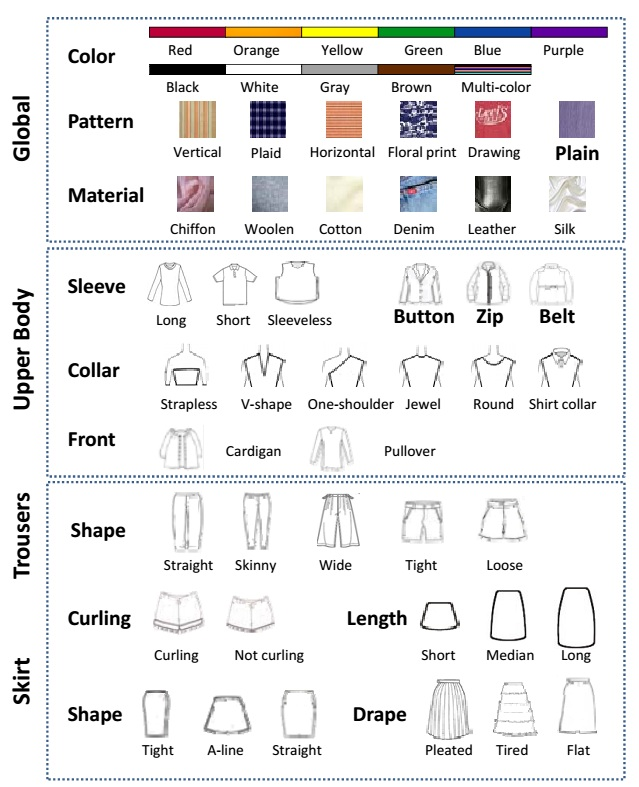
\includegraphics[width=0.9\textwidth]{img/attribute.jpg}
\caption{衣服属性示意图}
\label{fig:attribute}
\end{figure}

\subsection{衣服分类和匹配}
当进行完衣服属性分析后,我们相当于有了一个衣服属性的集合,这个集合里包含了所有的衣服属性(袖子、纹理、衣领等)信息。
首先我们的系统可以根据这些衣服属性对所有的衣服进行分类,每一个衣服属性都可以分很多类,比如袖子这个属性可以分为四类,长袖、中袖、短袖和无袖等。
这样可以为电商平台的服装商品构建一个强大的分类系统,用户根据这个分类系统也可以进行强大的检索行为。
其次,我们需要设计一个强大的、可伸缩的、精准的相似度匹配系统,来通过用户输入图片寻找最合适、最满足用户真实意图的衣服。
一个可行的方案是,将每件衣服都向量化为一个衣服属性特征向量,向量中包含了所有衣服属性信息。
这样我们可以通过标准的向量相似度函数来计算任意两个衣服属性特征向量的相似度。
从而对于用户输入的衣服图片,我们可以选择衣服数据库中相似度最接近的衣服,来推荐给用户。
这样节省了用户大量的时间,来进行搜索购买衣服。

\begin{figure}
\centering
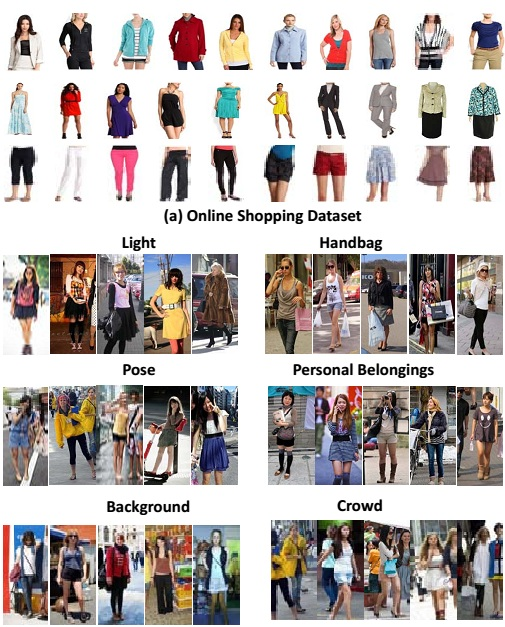
\includegraphics[width=0.9\textwidth]{img/map.jpg}
\caption{衣服属性与衣服匹配图}
\label{fig:attr-cloth}
\end{figure}

\section{基于图片的广告推荐}
广告是互联网时代最伟大的商业模式发明,它为互联网公司找到了流量变现的最强大方式。
从本质上来说,全球基本上所有的互联网公司都是广告公司,基本上百分之八十的收入都来自广告收入。
所以如何提高广告推荐的转化率,是互联网公司都需要面对的问题。
即就是将最精准的广告推送给用户,这个将极大的关乎到互联网公司的营收问题。

%图片

以前是文本广告推荐的模式,如今进入了图片时代,所以基于图片数据如何做广告推荐成为了一个新的挑战。
那我们专注在图片中包含人物的情况下,如何去做广告推荐。
广告是要产生商业价值的东西,所以我们尽可能去挖掘图片上所表达的语义信息,比如人做的动作,在进行斯诺克运动,那么我们可以推荐斯诺克球杆等,
比如人物所穿的衣服,我们可以根据衣服的属性样式去推荐类似的衣服,让用户产生购买的欲望需求。
所以本质上来说,基于图片的广告推荐也就是要去理解图片中表达的语义信息,只有理解了语义信息,才可以针对这些信息去做精准化的广告推荐。


\section{本章小结}
在本章中,我们看到了人体姿势预测任务的一些应用案例,有信息检索领域的、电子商务领域的、广告推荐领域的等。
可以看出,人体姿势预测是计算机视觉领域非常基础的一个问题,解决好了这个问题,那么就可以应用到很多相关领域。
而且我们可以看出,随着互联网的发展,文本数据的方式已经慢慢成熟,而图片时代将慢慢到来,但是文本数据时代积累的经典方法依旧值得我们采纳。
在处理图片数据时,我们还是去理解图片中包含的语义信息,并且可以借鉴文本数据时代的方法。
因此不同数据集上的方法可以是互相借鉴的,只不过处理的方式不同而已。
